\documentclass[thesis.tex]{subfiles}

\begin{document}
\chapter{Validation of the approach}
\label{sec:validation}
In the previous two chapters we have described the approach we developed and how we chose to implement it. This chapter is concerned with showing the behaviour of the approach. When a set of sequences are combined into a graph there should be an expectation as to what the result should look like. This expectation is grounded in the underlying formalism of the approach: The definitions of the involved elements, the scoring schema used and even smaller details like the order of some operations. We now increase the level of abstraction from the realm of formal details into "What results can we expect from using this approach".\\
\par\noindent
Throughout the chapter we will be doing example runs of the tool on some input data coupled with the actual graphical output. Additionally we will present some statements regarding the state of the data structures to represent the formalization of the expectation of the results. Importantly, this is not an attempt to show whether the tool acts correctly or not, that part is covered by the next chapter. This is a chapter determined to show the reader what it is we actually deem as correct behaviour, and how this behaviour is manifested through the input/output pairs. Throughout the development and implementation process these expectations and many more have been used as requirement specifications, realized through a test set which can be found in the github repo\footnote{Found in the presentation of the tool inAppendix \ref{sec:tool}}.\\
\par\noindent
The scoring schema used throughout the chapter is the negated edit distance scoring schema. This is used because of the intuituve results provided by the flat scoring structure. 
\section{Test data}
In order to avoid any ambiguity the test data in this chapter consists of small, hand-crafted sequences. As mentioned, the behaviour of the approach is determined by a relatively small set of formal instructions as to how it should behave in different circumstances. However, these instructions can be nested. This is a step which is cruical in order to produce graphs complex enough to fairly represent genetic variation. As the nesting goes on and the structures involved grow more and more complex, finding the underlying formal rules becomes non-trivial. The subsequent tests are divided into sections, the sequences in each section are designed to represent exactly one trait of genetic data which the algorithm should handle in a specific way.\\
\par\noindent
Although negated edit distance provide a good basis for intuitive results, the flat structure also presents a possible weakness: The scoring schema yields results which are susceptible to order of operations characteristics of the implementation. The test sequences provided are constructed to avoid any ambiguity concerning the order of the instructions given.
\section{Tests}
We start out with the most basic operation: Turning a sequence into a reference graph. The input sequence is given through the \texttt{-{}-input-sequences} argument. Throughout the chapter we will first show the command, or commands, which is run:\\
\par\noindent
\texttt{./build\_index.sh -{}-input-sequences=ACGTATTAC -{}-png=build}\\
\par\noindent
We will then show the graphical result which is stored in a png-file with the name given as a \texttt{-{}-png} argument:\\
\begin{figure}[!h]
  \begin{mdframed}
    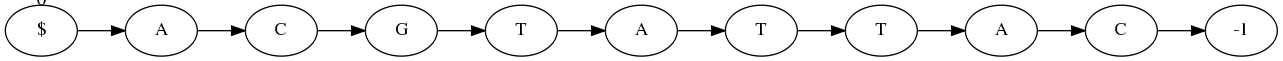
\includegraphics[width=\textwidth]{output/build.png} 
  \end{mdframed}
  \caption[A reference graph made from the sequence ``ACGTATTAC'']{The reference graph made from the sequence "ACGTATTAC"}
  \label{fig:validation_ref}
\end{figure}
\par\noindent
At last we provide a set of statements regarding the result:
\begin{itemize}
\item A reference graph made from a string $s$ should have exactly $|s|+2$ vertices
\end{itemize}
These statements are not exhaustive with regards to the output, as such a list would be very long and not particulary interesting. The statements provided will be what we classify as important details which follow from the inner workings of the algorithm, which in part means we omit statements which are exceedingly trivial.\\
\par\noindent
The graph built in this example will provide a basis for all of the following examples. In order to provide a working setup to readers who use this chapter as an introduction to the tool the different tests are separated by their index-file, determined by the \texttt{-{}-index} parameter, and the png filename.
\subsection*{Equal sequences}
We move on the the most trivial alignment operation, aligning a sequence against itself:\\
\par\noindent
\texttt{./build\_index.sh -{}-input-sequences=ACGTATTAC\\
-{}-index=equal.index}\\
\texttt{./align\_sequence.sh -{}-index=equal.index\\
-{}-align-sequence=ACGTATTAC -{}-png=equal-align}\\
\texttt{./align\_sequence.sh -{}-index=equal.index\\
-{}-align-sequence=ACGTATTAC -{}-merge=true -{}-png=equal-merge}\\
\begin{figure}[!h]
  \begin{mdframed}
  \begin{subfigure}[t]{\textwidth}
      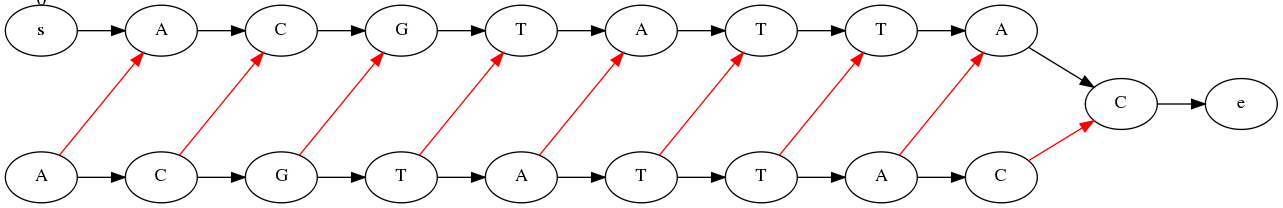
\includegraphics[width=\textwidth]{output/equal-align.png}
    \subcaption{}
  \end{subfigure}
  \begin{subfigure}[t]{\textwidth}
      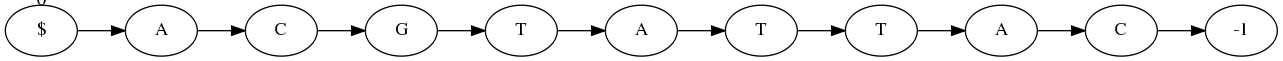
\includegraphics[width=\textwidth]{output/equal-merge.png}
    \subcaption{}
  \end{subfigure} 
  \end{mdframed}
  \caption[Aligning and merging an equal sequence into \ref{fig:validation_ref}]{The result of aligning (a) and merging (b) the sequence "ACGTATTAC" against the reference seen in figure \ref{fig:validation_ref}}
  \label{fig:validation_equal}
\end{figure}
\begin{itemize}
\item Aligning a sequence against itself should provide an alignment with the indexes of continuous vertices
\item Merging a sequence with itself should result in a graph with the same number of vertices as before the merge
\end{itemize}
\clearpage
\subsection*{SNPs}
We let SNPs be the first point mutation. At first we align and merge without setting the error margin $\lambda$:\\
\par\noindent
\texttt{./build\_index.sh -{}-input-sequences=ACGTATTAC\\
-{}-index=snp-no-errors.index}\\
\texttt{./align\_sequence.sh -{}-index=snp-no-errors.index\\
-{}-align-sequence=ACGGATTAC -{}-png=snp-no-errors-align}\\
\texttt{./align\_sequence.sh -{}-index=snp-no-errors.index\\
-{}-align-sequence=ACGGATTAC -{}-merge=true -{}-png=snp-no-errors-merge}\\
\begin{figure}[!h]
  \begin{mdframed}
  \begin{subfigure}[t]{\textwidth}
      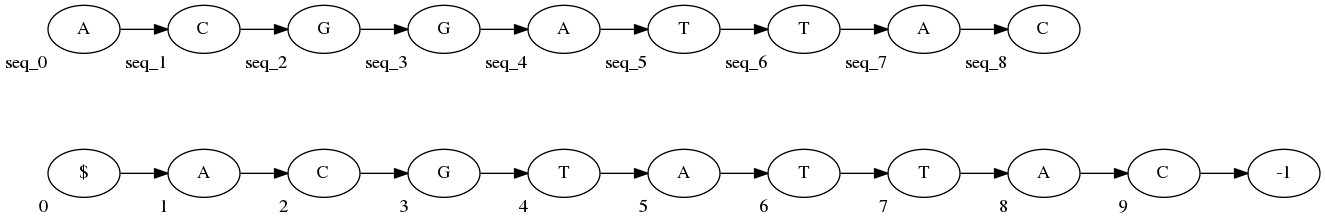
\includegraphics[width=\textwidth]{output/snp-no-errors-align.png}
    \subcaption{}
  \end{subfigure}
  \begin{subfigure}[t]{\textwidth}
      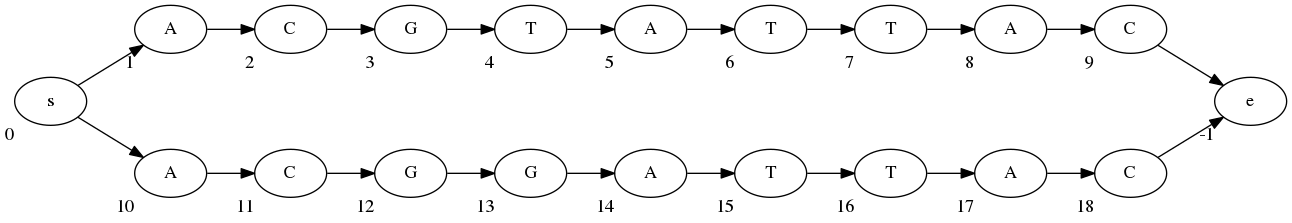
\includegraphics[width=\textwidth]{output/snp-no-errors-merge.png}
    \subcaption{}
  \end{subfigure}
  \end{mdframed}
  \caption[Aligning and merging an SNP with \ref{fig:validation_ref} with no error margin]{The result of aligning (a) and merging (b) the sequence "ACGTATTAC" against the reference seen in figure \ref{fig:validation_ref}}
  \label{fig:validation_snp_no_error}
\end{figure}
\begin{itemize}
\item Aligning a sequence with an error compared to the reference and no error margin should result in an empty alignment
\item Merging in an empty alignment should result in a new full path
\end{itemize}
\clearpage\noindent
We then align the same sequence while allowing an error margin through the \texttt{-{}-error-margin} parameter:\\
\par\noindent
\texttt{./build\_index.sh -{}-input-sequences=ACGTATTAC\\
-{}-index=single-snp.index}\\
\texttt{./align\_sequence.sh -{}-index=single-snp.index\\
-{}-align-sequence=ACGGATTAC -{}-error-margin=1 -{}-png=single-snp-align}\\
\texttt{./align\_sequence.sh -{}-index=single-snp.index\\
-{}-align-sequence=ACGGATTAC -{}-error-margin=1 -{}-merge=true \\
-{}-png=single-snp-merge}\\
\begin{figure}[!h]
  \begin{mdframed}
  \begin{subfigure}[t]{\textwidth}
      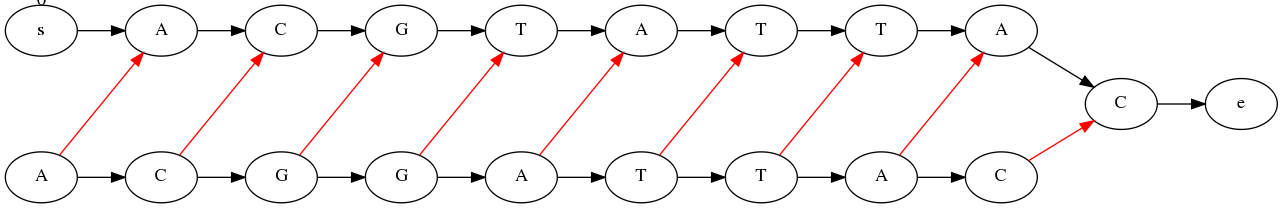
\includegraphics[width=\textwidth]{output/single-snp-align.png}
    \subcaption{}
  \end{subfigure}
  \begin{subfigure}[t]{\textwidth}
      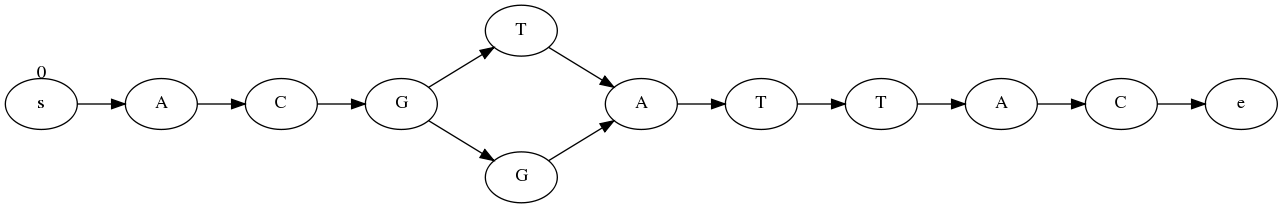
\includegraphics[width=\textwidth]{output/single-snp-merge.png}
    \subcaption{}
  \end{subfigure} 
\end{mdframed}
  \caption[Aligning and merging an SNP with \ref{fig:validation_ref} with a sufficient error margin]{The result of aligning (a) and merging (b) the sequence "ACGGATTAC" against the reference seen in figure \ref{fig:validation_ref}}
  \label{fig:validation_single_snp}
\end{figure}
\begin{itemize}
\item Aligning a sequence with a SNP compared to the reference should provide an alignment with the indexes of continuous vertices
\item Merging in a sequence with exactly one SNP should yield a graph with exactly one vertice more than the old graph, where exactly one vertice has one more outgoing edge and exactly one vertice has one more incoming edge.
\end{itemize}
\clearpage
\subsection*{Indels}
First we test a deletion by removing the fifth character in the alignment sequence:\\
\par\noindent
\texttt{./build\_index.sh -{}-input-sequences=ACGTATTAC \\
-{}-index=deletion.index}\\
\texttt{./align\_sequence.sh -{}-index=deletion.index \\
-{}-align-sequence=ACGTTTAC -{}-error-margin=1 -{}-png=deletion-align}\\
\texttt{./align\_sequence.sh -{}-index=deletion.index \\
-{}-align-sequence=ACGTTTAC -{}-error-margin=1 -{}-merge=true \\
-{}-png=deletion-merge}\\
\begin{figure}[!h]
  \begin{mdframed}
  \begin{subfigure}[t]{\textwidth}
      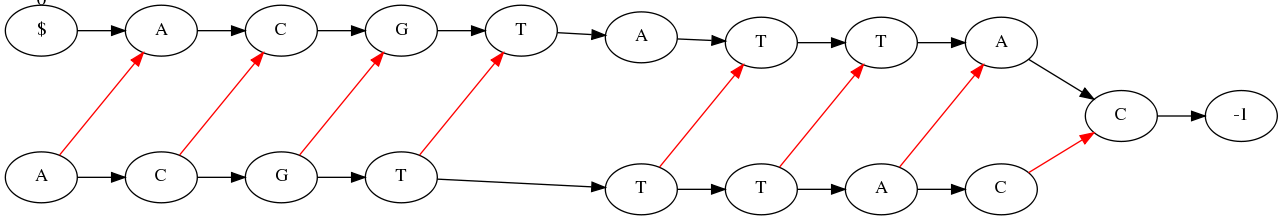
\includegraphics[width=\textwidth]{output/deletion-align.png}
    \subcaption{}
  \end{subfigure}
  \begin{subfigure}[t]{\textwidth}
      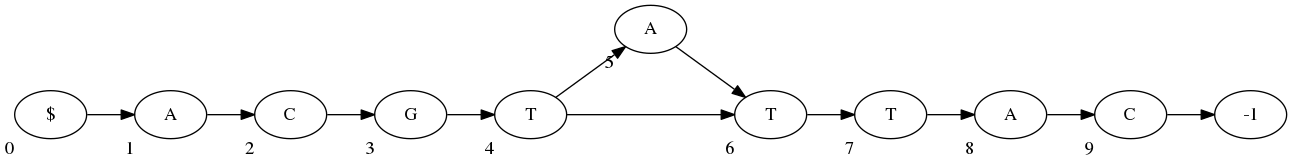
\includegraphics[width=\textwidth]{output/deletion-merge.png}
    \subcaption{}
  \end{subfigure}
  \end{mdframed}
  \caption[Aligning and merging a deletion with \ref{fig:validation_ref}]{The result of aligning (a) and merging (b) the sequence "ACGTTTAC" against the reference seen in figure \ref{fig:validation_ref}}
  \label{fig:validation_deletion}
\end{figure}
\begin{itemize}
\item Aligning a sequence with a deletion compared to the reference should provide an alignment where exactly one pair of consecutive indexes does not represent neighbouring vertices
\item Merging a sequence with a deletion should result in a graph with the same number of vertices as the old graph, but one additional edge
\end{itemize}
Secondly we test an insertion by inserting an extra 'A' after the fifth character:\\
\par\noindent
\texttt{./build\_index.sh -{}-input-sequences=ACGTATTAC \\
-{}-index=insertion.index}\\
\texttt{./align\_sequence.sh -{}-index=insertion.index \\
-{}-align-sequence=ACGTAATTAC -{}-error-margin=1 -{}-png=insertion-align}\\
\texttt{./align\_sequence.sh -{}-index=insertion.index \\
-{}-align-sequence=ACGTAATTAC -{}-error-margin=1 -{}-merge=true \\
-{}-png=insertion-merge}\\
\begin{figure}[!h]
  \begin{mdframed}
  \begin{subfigure}[t]{\textwidth}
      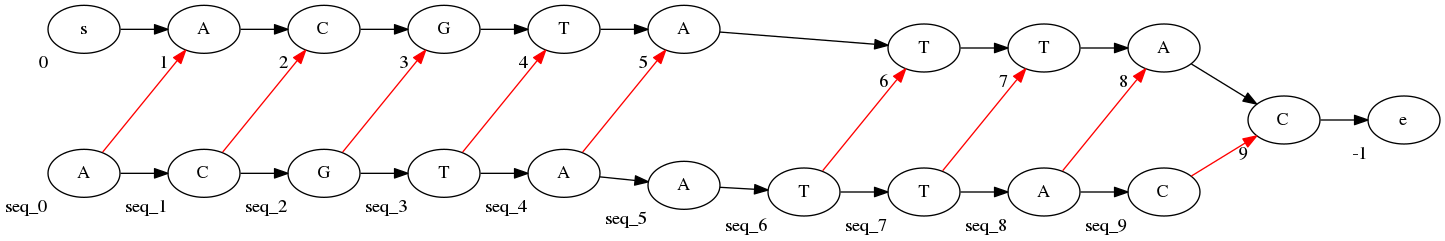
\includegraphics[width=\textwidth]{output/insertion-align.png}
    \subcaption{}
  \end{subfigure}
  \begin{subfigure}[t]{\textwidth}
      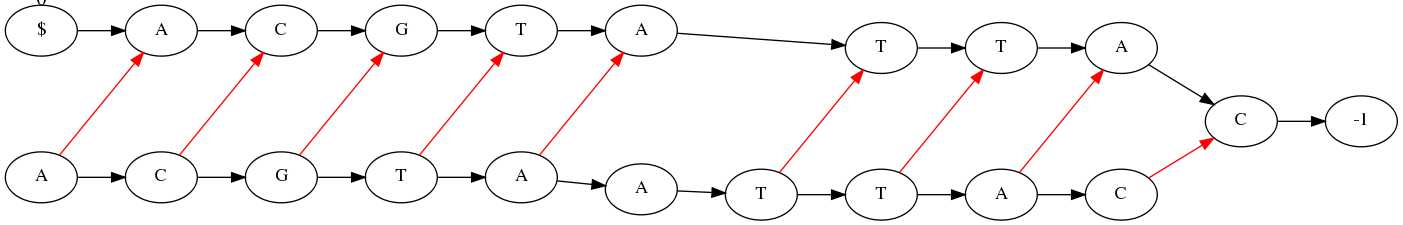
\includegraphics[width=\textwidth]{output/insertion-merge.png}
    \subcaption{}
  \end{subfigure} 
\end{mdframed}
  \caption[Aligning and merging an insertion with \ref{fig:validation_ref}]{The result of aligning (a) and merging (b) the sequence "ACGTAATTAC" against the reference seen in figure \ref{fig:validation_ref}}
  \label{fig:validation_insertion}
\end{figure}
\begin{itemize}
\item Aligning a sequence with an insertion compared to the reference should provide an alignment of indexes of consecutive vertices split apart by exactly one unmapped index
\item Merging a sequence with an insertion should result in a graph with exactly one more vertice and two more edges
\end{itemize}
\subsection*{Structural variation}
In section \ref{sec:genetic_variation} of the background chapter we present structural variation as mutations which occur over "larger areas of the genome". This kind of variation include larger subsequences which have been removed, inserted, moved or reversed. We can thus divide it into cases: In the case of removals we will see reads which span the sequence that is removed, represented by a large gap in corresponding path in the graph. This is a notion which does not go well with the strict mathematical notion of similarity, and is not handled well by the tool. However the approach does create data which could be useful in identifying such gaps\footnote{These are discussed as a part of the heuristical approach in \ref{sec:heuristical_conceptual} and \ref{sec:implementation_heuristic}}. In the case of a large insertion we will se reads which obviously does not have a counterpart in the graph. This will either result in unaligned reads or spurious matches with the most similar structure in the graph. Finding the true origin of these reads will have to be done by a larger assembly process\footnote{Briefly mentioned in \ref{sec:merge}}. Large subsequences which are moved will be similar to insertions, however here we will actually align the reads to their origin instead of having spurious results. Piecing them together correctly is also a job for an assembly process. The latter case of reversion is simply not implemented in the tool. This is not a result of laziness: It is done strictly in order to minimize the amount of ambiguity when showing the results achieved by the approach. Neither of the cases mentioned can be formulated like the small examples in this chapter, and is thus not shown.\\
\par\noindent
We will briefly treat structural variation as any variation which is not one of the point mutations depicted in the previous section. Conveniently, if we drop the actual large structural changes, these three mutations cover all the possible base cases of variation, and we can always define more complex cases as a combination of them. Because the number of possibilities grow exponentially we will only show a small fraction of cases in order to display the flexibilty of the approach.\\
\par\noindent
We start out by combining an insertion with an SNP:\\
\par\noindent
\texttt{./build\_index.sh -{}-input-sequences=ACGTATTAC \\
-{}-index=structural1.index}\\
\texttt{./align\_sequence.sh -{}-index=structural1.index \\
-{}-align-sequence=ACGTGGTTAC -{}-error-margin=2 -{}-merge=true \\
-{}-png=structural1-merge}\\
\begin{figure}[H]
  \begin{mdframed}
  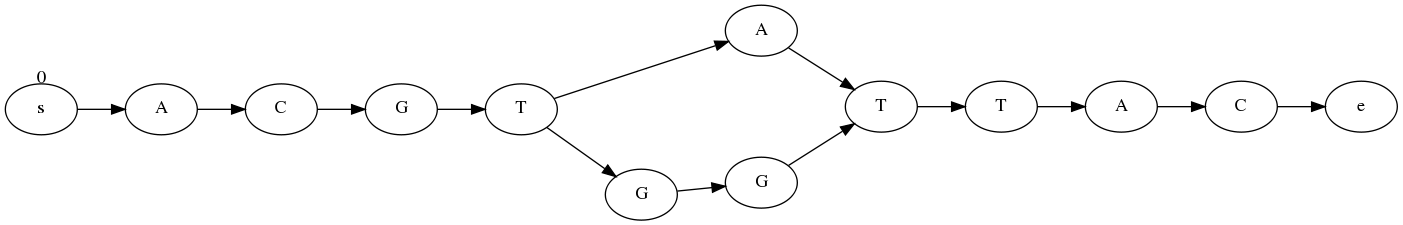
\includegraphics[width=\textwidth]{output/structural1-merge.png}
  \caption[Aligning and merging a complex variation with \ref{fig:validation_ref}]{The result of merging the sequence ``ACGTGGTTAC'' with the reference seen in figure \ref{fig:validation_ref}}
  \end{mdframed}
\end{figure}
\noindent
\begin{itemize}
  \item Merging in a sequence of length 10 should yield a graph with atleast one full path with length 12
\end{itemize}
When we are dealing with the "non-standard" cases we can see a statement which is \hlcyan{less exhaustive than earlier. This represent a correlation with the complexity of the input data: When the sequence consists of a combination of cases, so does the result. There is no longer a distinct relationship between a case and a rule, which can result in graphs which are not so easily deducible.} This becomes even more apparent when we align a sequence with a number of consecutive SNPs:\\
\par\noindent
\texttt{./build\_index.sh -{}-input-sequences=ACGTATTAC \\
-{}-index=structural2.index}\\
\texttt{./align\_sequence.sh -{}-index=structural2.index \\
-{}-align-sequence=ACGTACCTT -{}-error-margin=4 -{}-merge=true \\
-{}-png=structural2-merge}\\
\begin{figure}[H]
  \begin{mdframed}
  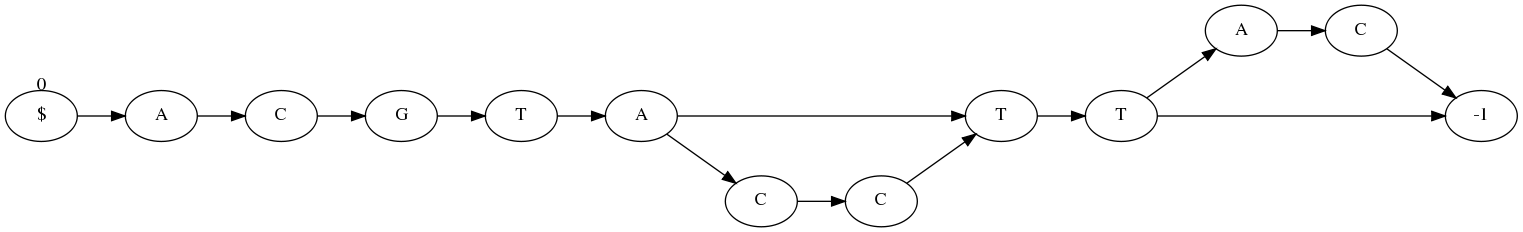
\includegraphics[width=\textwidth]{output/structural2-merge.png}
  \end{mdframed}
  \caption[Aligning and merging a second complex variation with \ref{fig:validation_ref}]{The result of merging the sequence ``ACGTACCTT'' with the reference seen in figure \ref{fig:validation_ref}}
\end{figure}
\noindent
At this point we do not achieve the result we expected. Instead of four SNPs the alignment contains two deletions and two insertions. Importantly, this is not a wrong result. The score for the alignment is exactly the same as the four SNPs we expected. This is a result of ambiguity created by the previously mentioned order of operations built in to the implementation. It is suboptimal that this kind of ambiguity exists, but it is a burden carried by the scoring schema and the problem definition rather than the approach itself.
\subsection*{Complex graphs}
In the last snippet of examples will be concerned with building more complex graphs. Although the previous examples are great displays of the basic functionality of the algorithm they don't exhibit the expressive power of the approach to any degree. This section will demonstrate this flexibility through a series of consecutive alignments and merges against the same graph and index.\\
\par\noindent
We start by building a graph from all the sequences from the first set of tests:\\
\par\noindent
\texttt{./build\_index.sh -{}-input-sequences=ACGTATTAC,ACGGATTAC,\\ACGTTTAC,ACGTAATTAC -{}-index=complex.index -{}-error-margin=1 \\-{}-png=complex1}\\
\par\noindent
\begin{figure}[H]
  \begin{mdframed}
  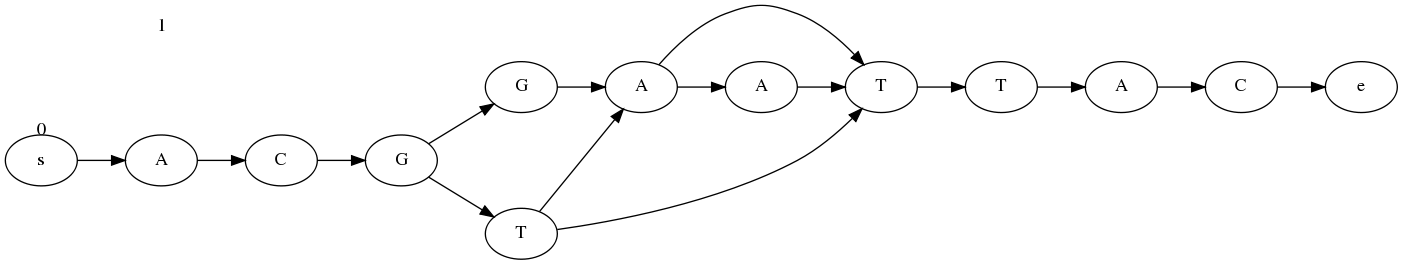
\includegraphics[width=\textwidth]{output/complex.png}
  \caption[A complex reference graph]{The reference graph made from the sequences ``ACGTATTAC'', "ACGGATTAC", ``ACGTTTAC'', ``ACGTAATTAC''}
  \label{fig:validation_complex_ref}
  \end{mdframed}
\end{figure}
\begin{itemize}
  \item All sequences used in building the graph has a corresponding full path
\end{itemize}
\noindent
We then merge in the sequences from the previous section:\\
\par\noindent
\texttt{./align\_sequence.sh -{}-index=complex.index \\
-{}-align-sequence=ACGTGGTTAC -{}-error-margin=2 -{}-merge=true}\\
\texttt{./align\_sequence.sh -{}-index=complex.index \\
-{}-align-sequence=ACGTACCTT -{}-error-margin=4 -{}-merge=true \\
-{}-png=complex-merge}\\
\begin{figure}[H]
  \begin{mdframed}
    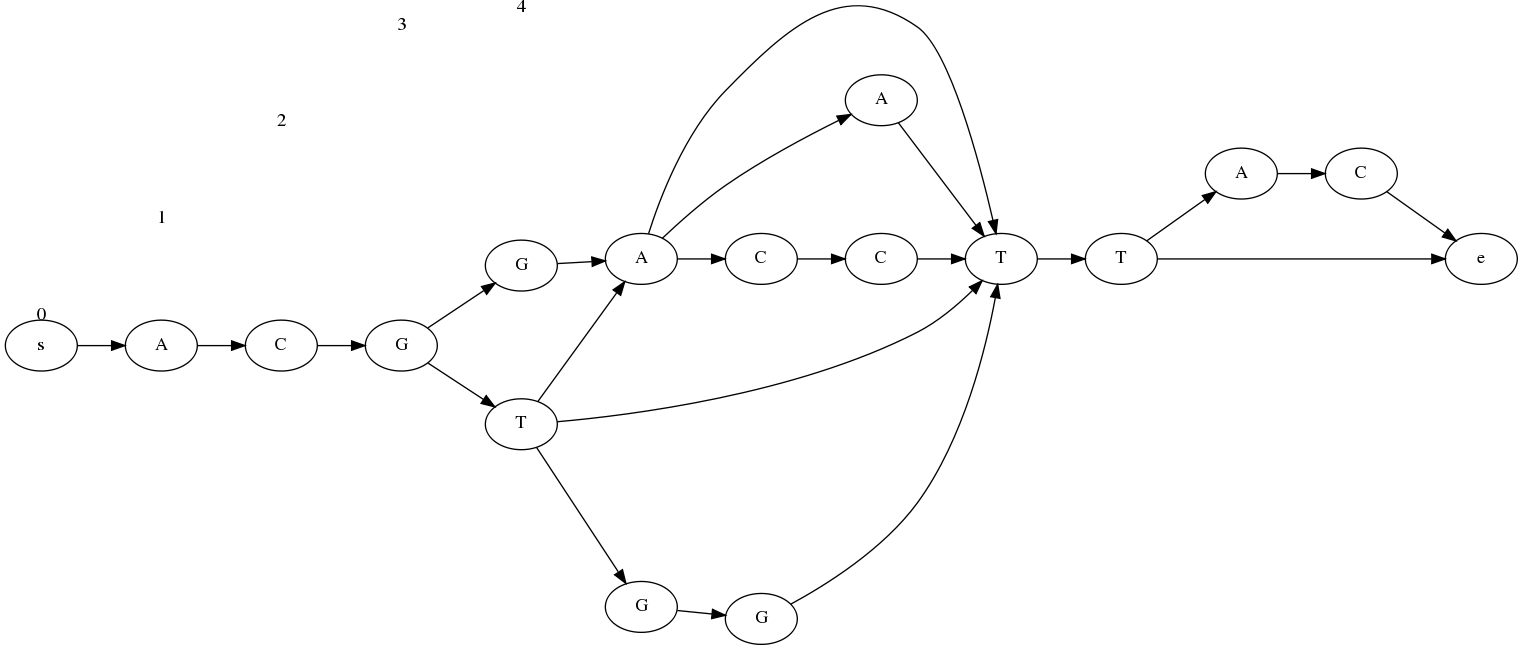
\includegraphics[width=\textwidth]{output/complex-merge.png}
  \end{mdframed}
  \caption[The result of merging several sequences into \ref{fig:validation_complex_ref}]{The two sequences ``ACGTGGTTAC'' and ``ACGTACCTT'' merged into the graph reference from figure \ref{fig:validation_complex_ref}}
  \label{fig:complex_2}
\end{figure}
\noindent
Although it is small, this is what we would consider to be an extremely complex graph in the domain of genetic information.\textcolor{red}{ The value of the graph based approach becomes apparent through the visualization: The variable genomic regions present themselves in a way which begs to be analyzed}. Because the graph is a result of several levels of complex nesting it is even harder to provide intuitive statements as to what it should look like. We can still depend on the definitions to provide them for us. For instance we can again expect every input sequence to have a full path. We can confirm this by aligning one of the sequences against the graph:
\clearpage\noindent
\texttt{./align\_sequence -{}-index=complex.index \\
  -{}-align-sequence=ACGTGGTTAC -{}-error-margin=0 \\
  -{}-png=complex-align}
\begin{figure}[H]
  \begin{mdframed}
    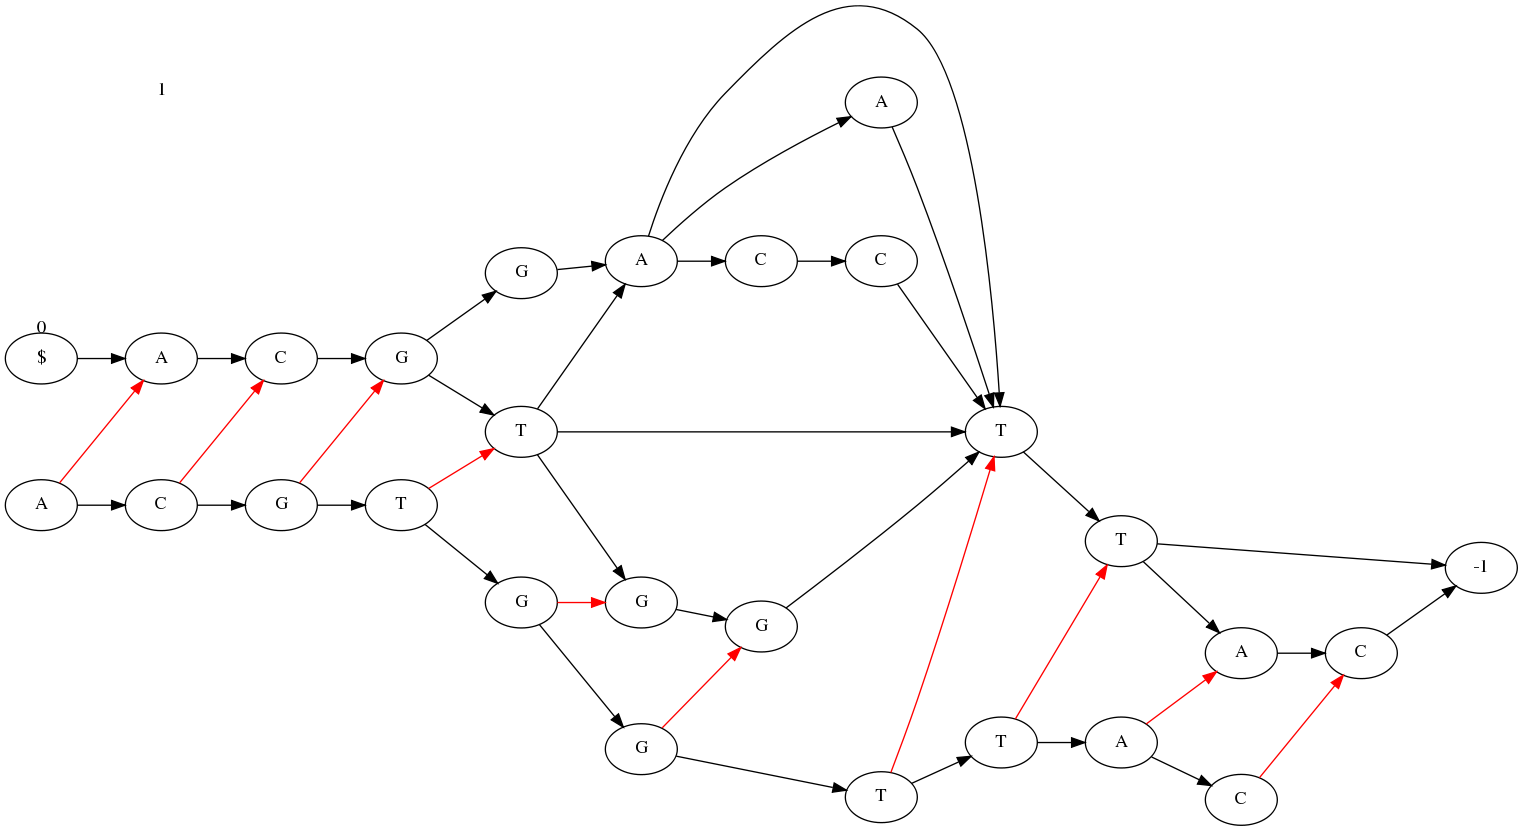
\includegraphics[width=\textwidth]{output/complex-align.png}
  \end{mdframed}
  \caption[Aligning a sequence against \ref{fig:complex_2}]{Aligning the sequence ``ACGTGGTTAC'' against the reference graph seen in figure \ref{fig:complex_2}}
\end{figure}
Because of the quick growth in complexity we will let this be the last visualized result. We will in the next chapter move on to large datasets and automated validation when testing the efficiency of the approach.
\end{document}